\begin{figure}[ht] 
 	\centering 
 	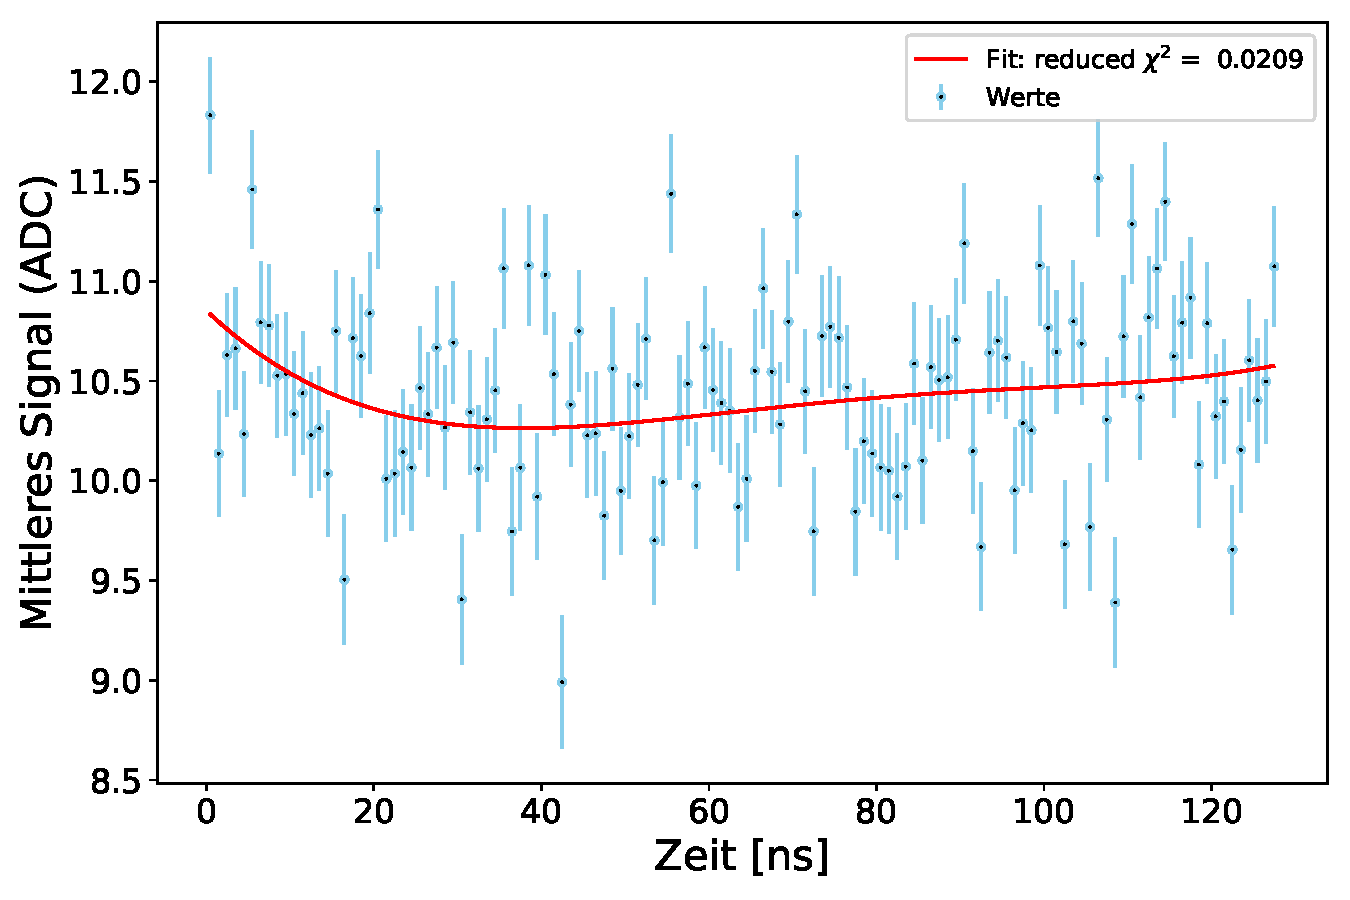
\includegraphics[width= 0.65 \textwidth]{Fits/A1_0V_Pedestals_Noise_Fit.pdf} 
	\caption{A1_0V_Pedestals_Noise, Fit} 
 	\label{fig:A1_0V_Pedestals_Noise, Fit} 
\end{figure}
 \\ 
\begin{align} 
 f(x) = a x^{4} + b x^{3} + c x^{2} + d x + e
\end{align} 
\begin{table}[ht] 
\centering 
\caption{A1_0V_Pedestals_Noise, Fit Parameter Tabelle} 
\label{tab:my-table}
\begin{tabular}{|l|c|}
\hline
Parameter Name	&	Wert \\ \hline
a	&	 2.4e-08 \pm  3.25e-08\\ \hline
b	&	-7.7849e-06 \pm  8.39e-06\\ \hline
c	&	 0.000897 \pm  0.000715\\ \hline
d	&	-0.039665 \pm  0.0226\\ \hline
e	&	 10.853 \pm  0.21\\ \hline
\end{tabular} 
\end{table}